\documentclass[aspectratio=169,10pt]{beamer}

% Import all packages
%%%%%%%%%%%%%%%%%%%%%%%%%%%%%%%
%     import des packages     %
%%%%%%%%%%%%%%%%%%%%%%%%%%%%%%%
\usepackage[export]{adjustbox}
\usepackage{amsmath,amsfonts,amssymb}
\usepackage{anyfontsize}
\usepackage{array}
\usepackage[french]{babel}
\usepackage{bbm}
\usepackage{colortbl}
\usepackage{comment}
\usepackage{cclicenses}
\usepackage{eqnarray}
\usepackage{eso-pic}
\usepackage{enumerate} % Pour personnaliser les énumération
\usepackage{fancybox}
\usepackage{fancyhdr}
\usepackage{float}
\usepackage[T1]{fontenc} 
\usepackage{forest}
\usepackage{gensymb}
\usepackage{geometry}
\usepackage{glossaries}
\usepackage{graphicx}
\usepackage{hyperref}
\usepackage{ifthen}
\usepackage{import}
\usepackage{indentfirst}
\usepackage[utf8]{inputenc}
\usepackage{lastpage}
\usepackage{libertine}
\usepackage{lipsum}
\usepackage{listings}
\usepackage{lmodern}
\usepackage{mathtools}
\usepackage{mdframed}
\usepackage{multicol}
\usepackage{pdfpages}
\usepackage{pifont}
\usepackage{stmaryrd}
\usepackage{subcaption}
\usepackage{subfiles}
\usepackage{tabularx}
% \usepackage{tcolorbox}
\usepackage[most]{tcolorbox}
\usepackage[absolute,overlay]{textpos} % To position the image
\usepackage{textcomp}
\usepackage{ulem}
\usepackage{wrapfig}
\usepackage{xcolor}


\newcommand{\titre}{Conception et optimisation d'algorithmes de coordination multi-robot}
\newcommand{\titrefooter}{Soutenance - Projet de fin d'études}
\newcommand{\soustitre}{Exploration autonome de réseaux de galerie}
\newcommand{\auteur}{Fabien MATHÉ}
\newcommand{\referent}{M. Mehmet ERSOY}
\newcommand{\institut}{Seatech - MOCA 3A}
\newcommand{\presentationdate}{27 février 2025}


% Thème clair et épuré
\usetheme{Berlin} % Thème Berlin
\usecolortheme{seahorse}
\setbeamertemplate{navigation symbols}{} % Suppression des symboles de navigation

% Personnalisation du thème

% Couleurs personnalisées
\definecolor{mainblue}{RGB}{0, 102, 204} % Bleu principal
\definecolor{lightgray}{RGB}{240, 240, 240} % Gris clair
\definecolor{darkgray}{RGB}{100, 100, 100} % Gris plus foncé pour les points non actifs
\definecolor{lightblue}{RGB}{173, 216, 230} % Bleu clair
\definecolor{darkblue}{RGB}{0, 51, 102} % Bleu foncé

% Configuration des couleurs
% \setbeamercolor{normal text}{bg=white, fg=black}
% \setbeamercolor{structure}{fg=mainblue}
% \setbeamercolor{frametitle}{bg=lightgray, fg=mainblue}
% \setbeamercolor{title}{fg=mainblue}
% \setbeamercolor{itemize item}{fg=mainblue}

% Personnalisation des couleurs du thème
\setbeamercolor{normal text}{bg=white, fg=black} % Texte principal en gris foncé sur fond blanc
\setbeamercolor{structure}{fg=mainblue} % Couleur principale des titres (sections, sous-sections)
\setbeamercolor{frametitle}{bg=lightgray, fg=mainblue} % Titre des frames avec fond bleu clair et texte bleu
\setbeamercolor{title}{fg=mainblue} % Couleur du titre principal
\setbeamercolor{itemize item}{fg=mainblue} % Couleur des puces (items)
\setbeamercolor{enumerate item}{fg=mainblue} % Couleur des items des listes numérotées
\setbeamercolor{section in toc}{fg=mainblue} % Sections dans la table des matières
\setbeamercolor{subsection in toc}{fg=darkblue} % Sous-sections dans la table des matières

% Personnalisation des blocs de couleur
\setbeamercolor{block title}{bg=mainblue, fg=white} % Titre des blocs avec fond bleu et texte blanc
\setbeamercolor{block body}{bg=lightblue, fg=black} % Corps des blocs avec fond bleu clair et texte noir
\setbeamercolor{alertblock title}{bg=darkblue, fg=white} % Titre des alertes avec fond bleu foncé et texte blanc
\setbeamercolor{alertblock body}{bg=lightblue, fg=black} % Corps des alertes avec fond bleu clair et texte noir
\setbeamercolor{exampleblock title}{bg=mainblue, fg=white} % Titre des exemples avec fond bleu et texte blanc
\setbeamercolor{exampleblock body}{bg=lightblue, fg=black} % Corps des exemples avec fond bleu clair et texte noir

% \setbeamercolor{palette primary}{use=structure,fg=white,bg=structure.fg}
% \setbeamercolor{palette secondary}{use=structure,fg=white,bg=structure.fg!75}
% \setbeamercolor{palette tertiary}{use=structure,fg=white,bg=mainblue}
% \setbeamercolor{palette quaternary}{fg=white,bg=mainblue}

% Modification des puces (bulles) dans les listes
\setbeamertemplate{itemize item}[circle] % Change les puces classiques en cercles
%\setbeamertemplate{itemize item}[square] % Change les puces en carrés
%\setbeamertemplate{itemize item}[triangle] % Change les puces en triangles
%\setbeamertemplate{itemize item}[rectangle] % Change les puces en rectangles

% Modification des numéros dans les listes numérotées (enumerate)
\setbeamertemplate{enumerate item}[circle] % Change les numéros en cercles
%\setbeamertemplate{enumerate item}[square] % Change les numéros en carrés
%\setbeamertemplate{enumerate item}[triangle] % Change les numéros en triangles
%\setbeamertemplate{enumerate item}[rectangle] % Change les numéros en rectangles


% Bas de page personnalisé (nom, établissement, date, numéro de page)
\newcommand{\customfootline}{
	\setbeamertemplate{footline}{
		\begin{beamercolorbox}[ht=2ex, dp=1ex]{}
			\colorbox{lightgray}{
				\parbox{\textwidth}{
					\begin{minipage}{0.19\linewidth}
						\centering
						\auteur
					\end{minipage}
					\hfill
					\begin{minipage}{0.19\linewidth}
						\centering
						\institut
					\end{minipage}
					\hfill
					\begin{minipage}{0.19\linewidth}
						\centering
						\titrefooter
					\end{minipage}
					\hfill
					\begin{minipage}{0.19\linewidth}
						\centering
						\presentationdate
					\end{minipage}
					\hfill
					\begin{minipage}{0.19\linewidth}
						\centering
						\insertframenumber/\inserttotalframenumber
					\end{minipage}
					\vspace{0.5em}
				}
			}
		\end{beamercolorbox}
	}
}


% Titre de la présentation
\title[Titre court]{\titre}
\subtitle{\soustitre}
\author{\auteur}
\institute{\institut \newline \titrefooter}
\date{\presentationdate}

\usefonttheme[onlymath]{serif}

\begin{document}

% Page de titre (Timeline non affichée ici)

\setbeamertemplate{headline}{}
\setbeamertemplate{footline}{}

\begin{frame}
    \titlepage
\end{frame}

\setbeamertemplate{headline}[miniframes theme]
\customfootline

% Section 1 : Introduction
\section{Introduction}

\begin{frame}{\textbf{Introduction}}
	\begin{minipage}{0.6\linewidth}
		\begin{itemize}
			\item Fascination pour l'inconnu
			\vspace{0.2cm}
			\item Meilleure compréhension de notre planète
			\vspace{0.2cm}
			\item Défis inhérents de l'exploration souterraine
			\begin{itemize}
				\item Accessibilité
				\vspace{0.2cm}
				\item Communication
				\vspace{0.2cm}
				\item Navigation
			\end{itemize}
			\vspace{0.2cm}
			\item Intérêt scientifique
			\begin{itemize}
				\item Découverte de nouvelles formes de vie
				\vspace{0.2cm}
				\item Structures géologiques préservées
			\end{itemize}
		\end{itemize}
	\end{minipage}
	\hfill
	\begin{minipage}{0.35\linewidth}
		\begin{figure}
			\centering
			\includegraphics[width=0.8\textwidth]{IMAGES/Grotte_de_la_flûte_de_pan.jpeg}
			\caption{Grotte de la flûte de pan (Guilin, Chine). Paul Munhoven \href{https://commons.wikimedia.org/w/index.php?curid=27712205}{\copyright}}
			\label{fig:china_cave}
		\end{figure}
	\end{minipage}

\end{frame}

\begin{frame}{\textbf{Introduction}}

	\begin{minipage}{0.6\linewidth}
		\begin{figure}
			\centering
			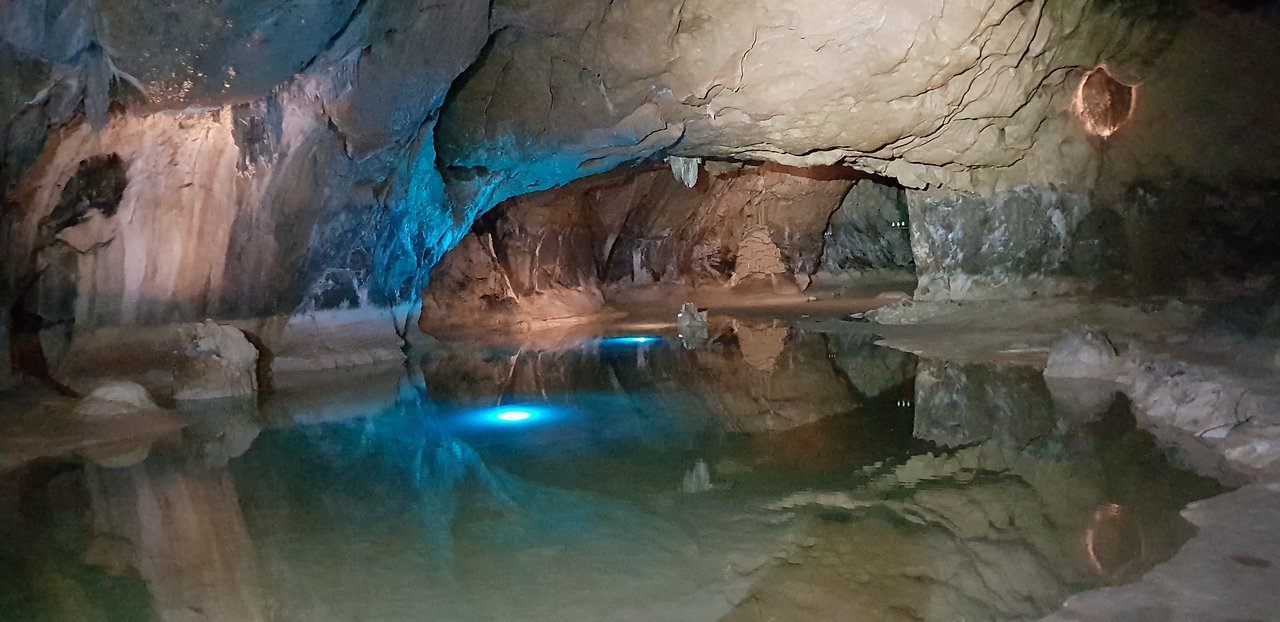
\includegraphics[width=0.8\textwidth]{IMAGES/le-lac-des-grottes-lombrives.jpg}
			\caption{Lac de la Grotte de Lombrives - Ariège}
			\label{fig:ariege_cave}
		\end{figure}
	\end{minipage}
	\hfill
	\begin{minipage}{0.35\linewidth}
		\begin{figure}
			\centering
			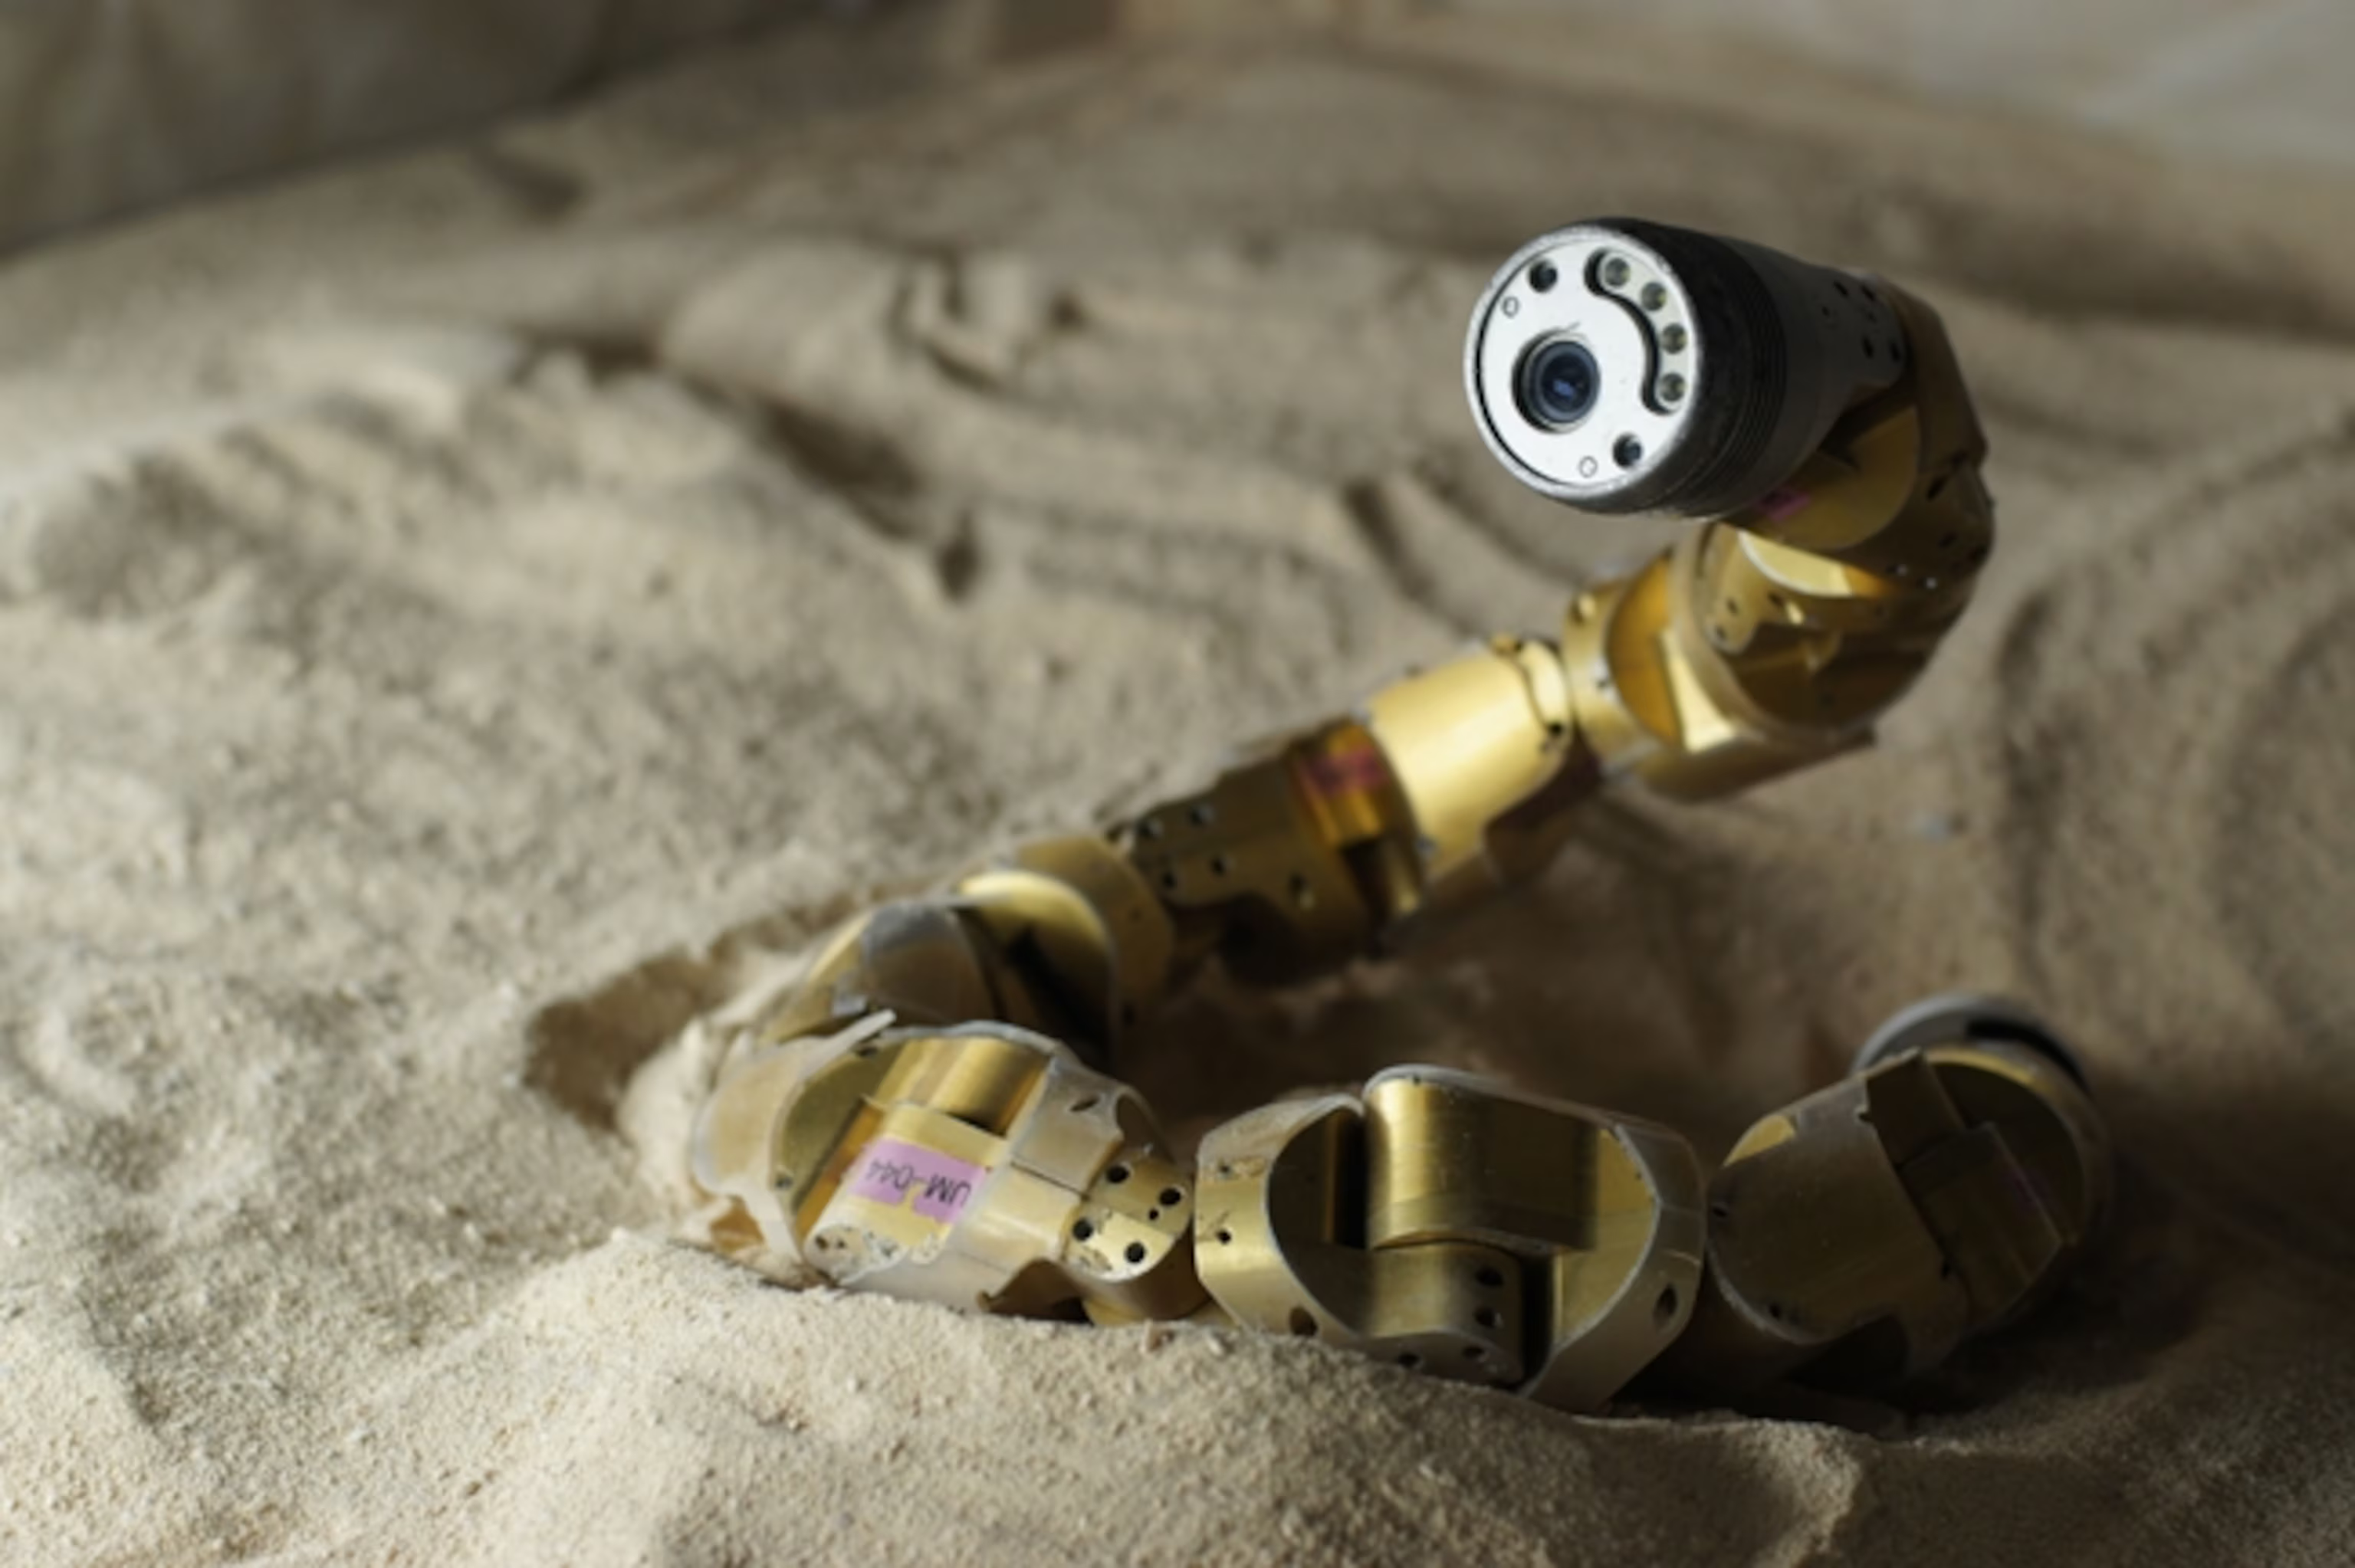
\includegraphics[width=0.9\textwidth]{IMAGES/Elizabeth.png}
			\caption{Elizabeth, le robot serpent. Nico Zevalios and Chaohui Gong}
			\label{fig:robot_exploration}
		\end{figure}
	\end{minipage}
    
	\textbf{Objectif :}

	\vspace{0.8em}
	\begin{itemize}
		\item Développer des algorithmes de navigation pour des robots autonomes en milieu souterrain.
		\vspace{0.2cm}
		\item Assurer une communication autonome entre des robots sans contrôle externe.
	\end{itemize}
\end{frame}

% Table des matières
\begin{frame}{\textbf{Sommaire}}
    \tableofcontents
\end{frame}




%%%%%%%%%%%%%%%%%%%%%%%%%%%%%%%%%%%%%%%%%%%%%%%%%%%%%%%%%%%%%%%%%%%%%%%%%%%%%%%%
% Section 2
%%%%%%%%%%%%%%%%%%%%%%%%%%%%%%%%%%%%%%%%%%%%%%%%%%%%%%%%%%%%%%%%%%%%%%%%%%%%%%%%
\section{Plannification de trajectoire}

\begin{frame}{\textbf{Tentative de d'optimisation théorique}}
	\begin{itemize}
		\item Objectif : Trouver le plus court chemin liant deux points
		\vspace{0.2cm}
		\item Contraintes :
		\vspace{0.2cm}
		\begin{itemize}
			\item Découverte dynamique de la carte
			\vspace{0.2cm}
			\item Évitement des obstacles
		\end{itemize}
		\vspace{0.2cm}
		\item Simplification :
		\vspace{0.2cm}
		\begin{itemize}
			\item Aucune contrainte liée au robot
			\vspace{0.2cm}
			\item Espace 2D
		\end{itemize}
	\end{itemize}
	% \begin{textblock*}{3cm}(12cm,3cm) % {block width} (coords)
	% 	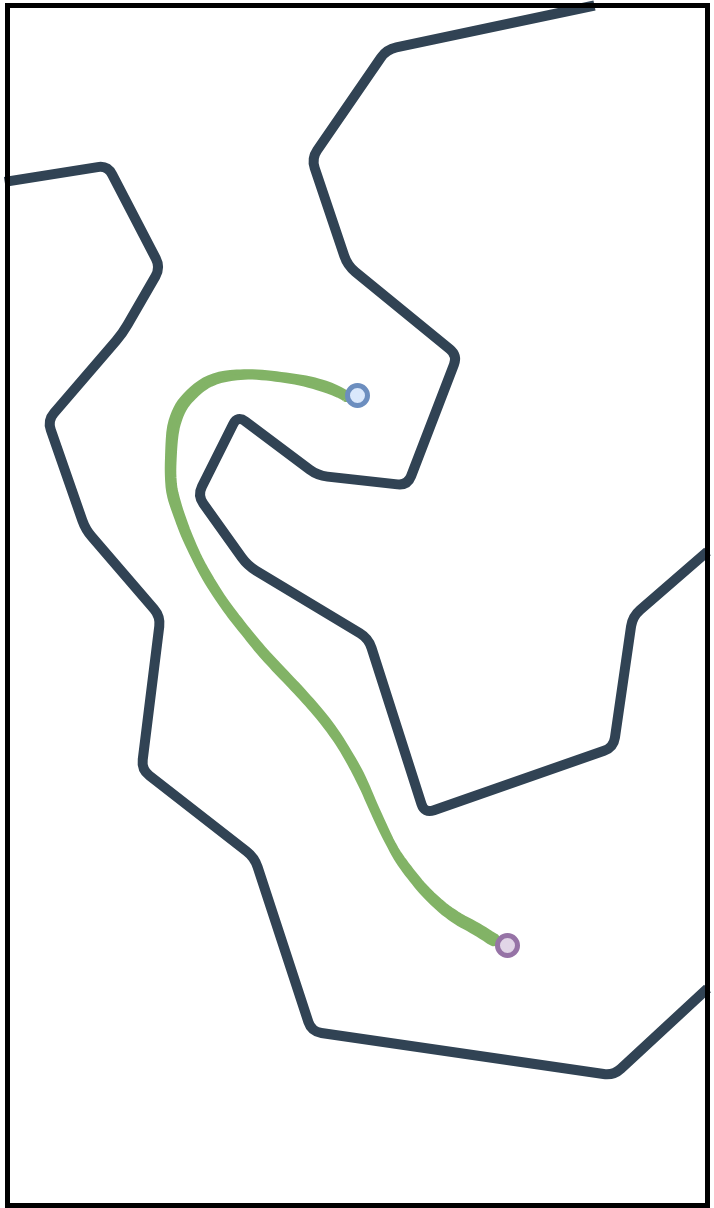
\includegraphics[width=3cm]{IMAGES/path_diagram_ilustration.png}
	% \end{textblock*}
	
\end{frame}

\begin{frame}[t]{\textbf{Définition de l'espace étoilé et de la fonctionnelle à optimiser}}
	\begin{minipage}[t]{0.6\linewidth}
		\begin{equation*}
			\displaystyle
			FV(t) = \left\{ \, (1 - l) \, \mathbf{X}(t) + l\, \mathbf{M}(t, \alpha) \,|\, l \in [0, 1], \alpha \in [0, 2 \pi[ \, \right\}
		\end{equation*}
			
		\begin{equation*}
			\mathbf{M}(t, \alpha) = \mathbf{X}(t) + R(t, \alpha) 
			\begin{pmatrix}
				\cos \alpha & 0\\
				0 & \sin \alpha\\
			\end{pmatrix} 
			\mathbf{X}(t)
		\end{equation*}

	Avec $R(t, \alpha)$ la distance minimale entre le robot et le plus proche point d'intersection à un mur, borné par $R_{\max}$.
	\end{minipage}
	\hfill
	\begin{minipage}[t]{0.38\linewidth}
		\begin{figure}
			\centering
			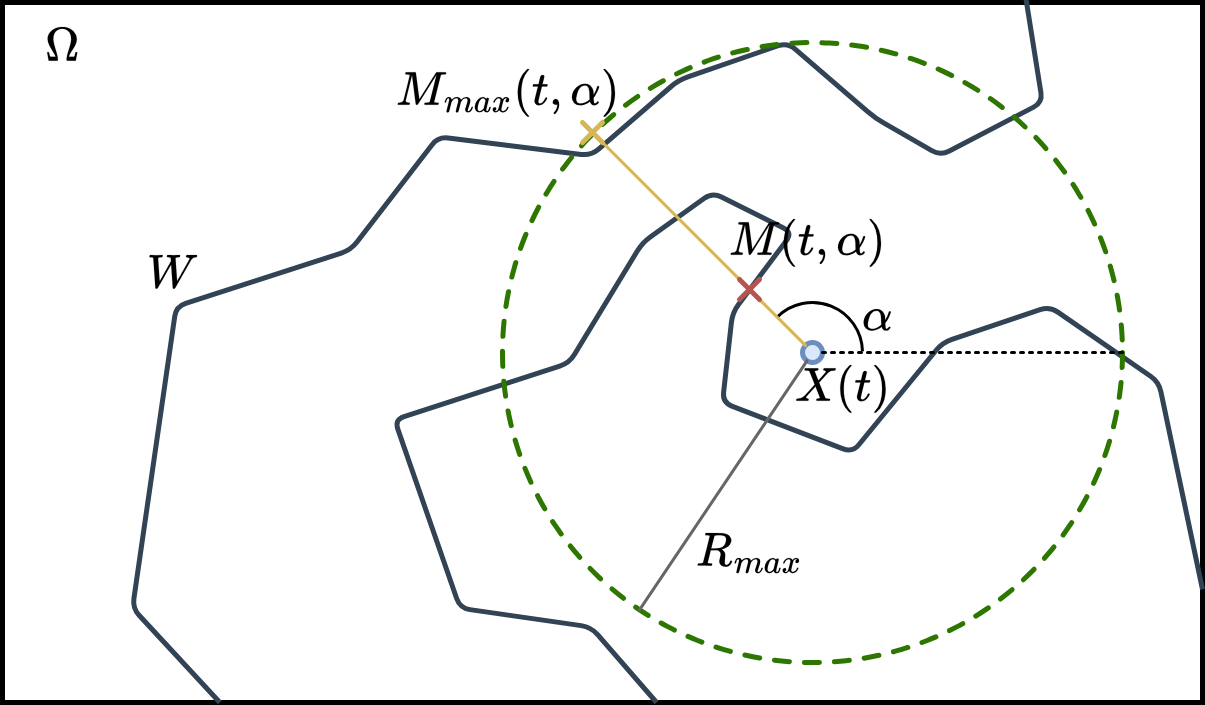
\includegraphics[width=\textwidth]{IMAGES/math_nota.png}
			\caption{Schéma des notations}
			\label{fig:math_notation}
		\end{figure}
	\end{minipage}

	\textbf{Fonctionnelle :}
	\begin{equation*}
		\displaystyle
		J(\mathbf{X}(0), T) = \int_{0}^{T} \| \mathbf{\dot{X}}(t) \| dt
	\end{equation*}
	avec $\mathbf{X}(0) = \mathbf{X}_{Robot}$ et $\mathbf{X}(T) = \mathbf{X}_{WP}$
	
\end{frame}

\begin{frame}{\textbf{Problèmes rencontrés}}
	Question ouverte :
		Comment garantir $\mathbf{X}(T)=\mathbf{X}_{WP}$ en contraignant $\dot{X}(t)$ ?
		Comment choisir le temps T ?
	
			Tdoit être suffisamment grand pour atteindre la cible.
			Si le robot s'arrête à $t_1$, alors :
			$\int_{t_1}^{t} \mathbf{X}(t)^{2} dt = 0$.
	
		Comment prendre en compte l'exploration de la carte ?

	Reduction du problème à une première approche simple supposant que la carte est connue.

\end{frame}

\begin{frame}{\textbf{Proposition d'une nouvelle méthode}}
    Slide 5
\end{frame}

\begin{frame}{\textbf{Méthode de vérification}}
    Slide 5
\end{frame}

\begin{frame}{\textbf{Méthode de vérification}}
    Slide 5
\end{frame}

\begin{frame}{\textbf{Résultats et performance}}
    Slide 5
\end{frame}

\begin{frame}{\textbf{Résultats et performance}}
    Slide 5
\end{frame}

% Section 3 : Résultats
\section{Communication}

\begin{frame}{\textbf{Résultats}}
    Slide 5
\end{frame}

\begin{frame}{\textbf{Résultats}}
    Slide 6
\end{frame}

\begin{frame}{\textbf{Résultats}}
    Slide 7
\end{frame}

\begin{frame}{\textbf{Résultats}}
    Slide 8
\end{frame}

\begin{frame}{\textbf{Résultats}}
    Slide 9
\end{frame}

% Section 4 : Discussions
\section{Simulateur et résultats}

\begin{frame}{\textbf{Discussions}}
    Slide 10
\end{frame}

\begin{frame}{\textbf{Discussions}}
    Slide 11
\end{frame}


% Section 5 : Conclusion
\section{Conclusion et perspectives}
\begin{frame}{\textbf{Conclusion}}
    Slide 12
	Un simulateur construit:
		Environ 3500 lignes de code
		Une dixaine de fonction utiles pour la suite
\end{frame}

% Section 5 : Conclusion
\begin{frame}{\textbf{Perspectives}}
    Slide 12
\end{frame}

\begin{frame}{\textbf{Perspectives}}
    Slide 13
\end{frame}

\begin{frame}{\textbf{Références}}
    Slide 13
\end{frame}

\end{document}
